\section*{Introduction}


Cloud Detection and Response (CDR) systems are essential for identifying threats in cloud environments, where worker nodes across a cloud cluster generate extensive audit logs that are centrally collected and analyzed. In a typical CDR workflow, these logs are gathered at a central point to detect suspicious activity, using either signature-based or anomaly-based detection methods. Signature-based methods \cite{elasticdetectionrules,chronicledetectionrules} rely on matching known threat patterns, which limits them to detecting established attacks. Anomaly-based methods \cite{aljawarneh2018anomaly,cai2021structural}, however, detect deviations from typical behavior, making them better suited for identifying novel and evolving threats.

\begin{wrapfigure}{R}{.35\linewidth}
    \centering 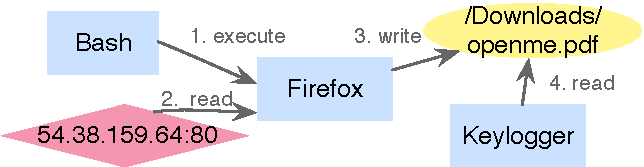
\includegraphics[width=0.35\textwidth]{fig/example.pdf}
    \caption{An example provenance graph showcasing the downloading of a malicious file. }
    \label{fig:example:provenance}
    \vspace{-2ex}
\end{wrapfigure}

Recent advances in anomaly detection leverage provenance techniques \cite{yangprographer,flash2024,cheng2023kairos}, which build data provenance graphs from audit logs to track sequences of related events. In these graphs, nodes represent system entities like processes or files, and edges depict system calls, such as read or fork, that define interactions between entities, as shown in Figure~\ref{fig:example:provenance}. Analyzing these graphs enables systems to detect complex, multi-step malicious behaviors that traditional methods might miss. This approach improves detection by identifying subtle, evolving attack patterns, allowing machine learning models trained on benign patterns to flag anomalies signaling potential threats.



Unfortunately, centralized CDR systems that rely on Security Information and Event Management (SIEM) platforms face significant challenges in scalability and efficiency within cloud clusters. SIEM systems typically aggregate and store massive volumes of audit logs from distributed worker nodes. When alerts are generated, Security Operations Centers (SOCs) must investigate by writing complex queries, often in languages like Kusto Query Language (KQL), to extract relevant data from these logs. This manual process is time-intensive, requires substantial expertise, and is prone to human error, especially as analysts interpret complex relationships within provenance graphs to distinguish benign from malicious behavior. Additionally, centralizing audit logs for processing creates data bottlenecks, network congestion, and delays in response times, ultimately slowing SOC operations and leaving incidents unresolved.

This proposal addresses these challenges with two main objectives. First, we will develop \Sysa, a decentralized detection system leveraging Federated Learning (FL) to enhance threat detection while minimizing centralized data transfers. \Sysa enables worker nodes to process audit logs locally, supporting scalable, cloud-native detection without the network overhead of centralized systems (Task~\ref{task:1}). Integrating FL into CDR systems presents challenges due to the heterogeneous, non-IID log distributions across nodes, leading to conflicting updates that degrade model performance \cite{bonawitz2019towards} and data imbalances that skew outcomes and reduce accuracy \cite{guo2023new,zhao2018federated}.

To overcome these issues, we combine FL with Graph Neural Networks (GNNs) to enable decentralized training directly on provenance graphs from worker nodes, removing the need for raw data sharing. Our approach introduces a novel FL aggregation algorithm with layer-wise coefficients to capture latent proximities among local updates, refined through confidence-based entropy minimization on proxy datasets. This system will incorporate worker-specific aggregation, adaptive learning rates, and asynchronous updates for faster model convergence. We will explore GNN architectures like GraphSAGE~\cite{lo2022graphsage} to capture structural and temporal interactions in provenance graphs, allowing for the detection of multi-step attacks. Additionally, attention mechanisms~\cite{vaswani2017attention} and Spatio-Temporal Graph Networks~\cite{yu2017spatio} will enhance embedding precision and capture evolving patterns, making \Sysa a scalable, cloud-native alternative to traditional CDR by minimizing centralized data transfer.

Secondly, we introduce \Sysb, an AI-driven SOC assistant that automates the generation of investigation queries for SIEM systems. Using a pre-trained language model (LLM), \Sysb interprets SOC investigation prompts to generate precise, contextually relevant queries. This process involves parsing the prompt to identify key data fields and entities, constructing a structured query, and refining it through an iterative, confidence-based review. By automating query generation, \Sysb enables SOC teams to conduct faster, more accurate investigations, bridging expertise gaps and streamlining response workflows (Task~\ref{task:2}).







% \begin{wrapfigure}{L}{.40\linewidth}
\begin{figure}[t!]
    \centering 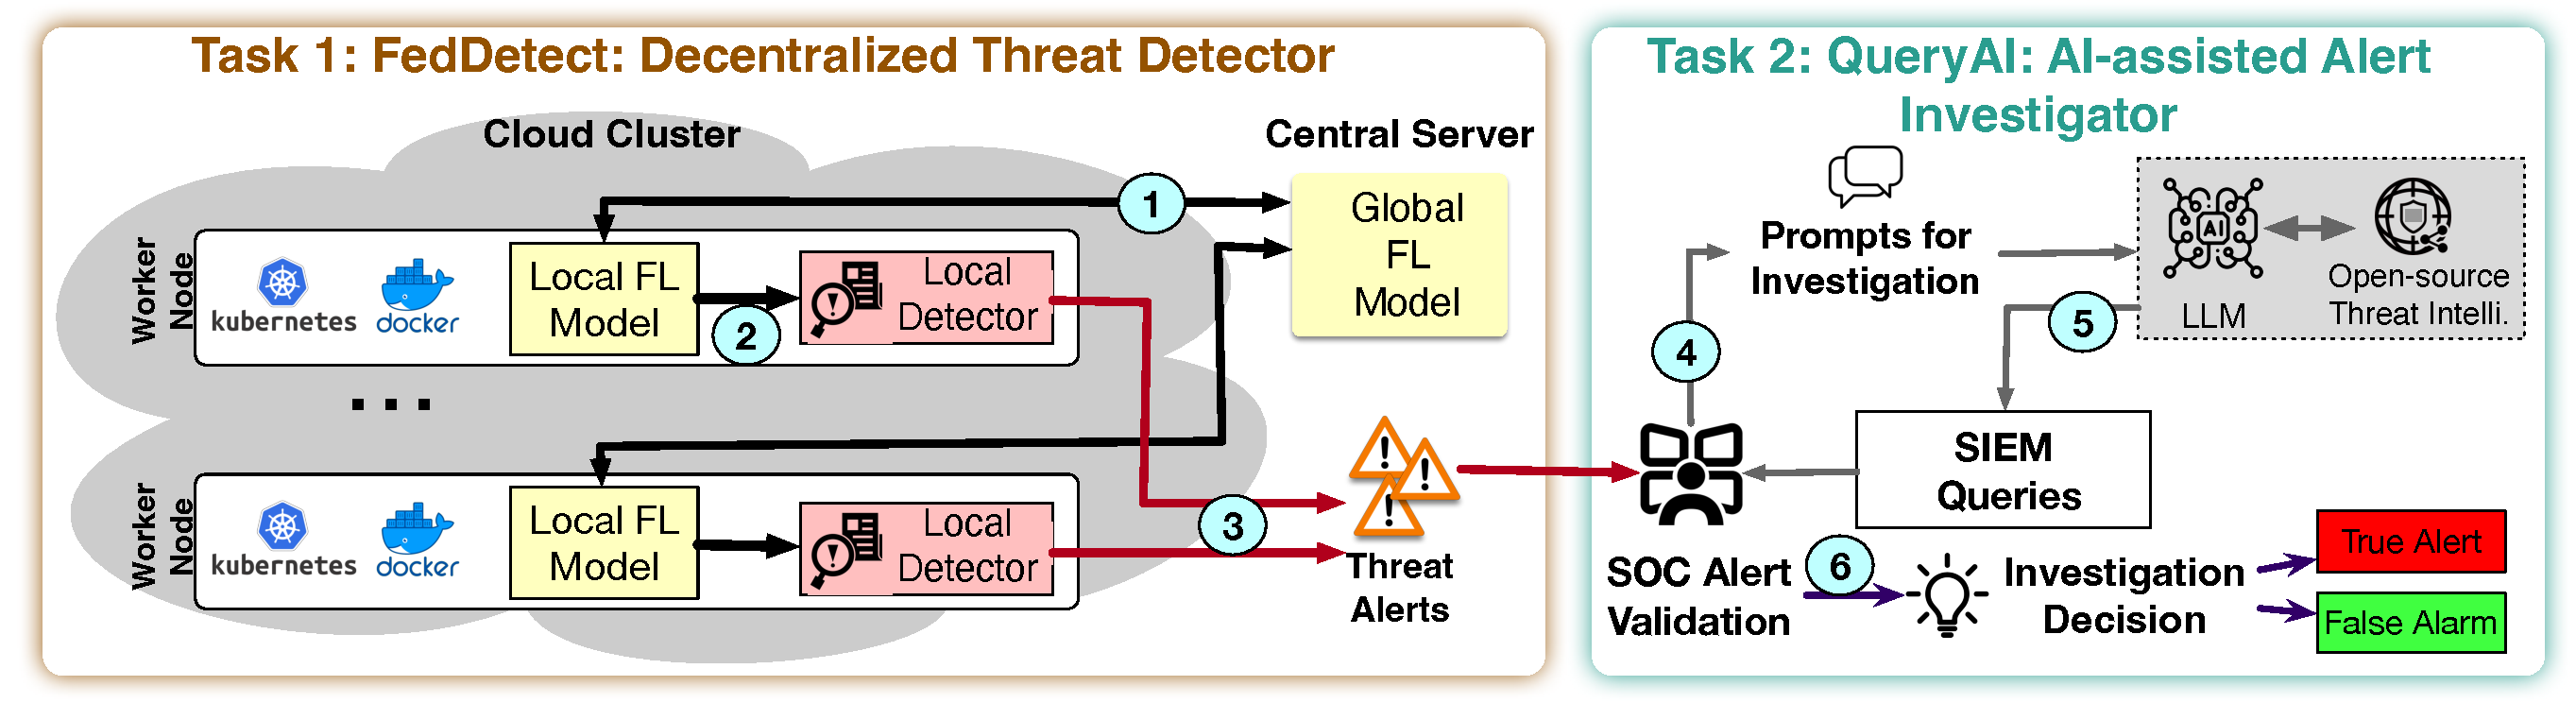
\includegraphics[width=0.80\textwidth]{fig/arch-e2e-cdr.pdf}
    \caption{Workflow of our proposed decentralized threat detector and AI-assisted alert investigation framework. }
    \label{fig:arch}
    \end{figure}
% \end{wrapfigure}



\noindent\textbf{PI Qualifications: }
PI Hassan is a leader in provenance-based system auditing and threat detection. His work includes developing methods for capturing audit logs from large-scale systems in a highly storage- and network-efficient manner~\cite{winnower2018,omegalog2020,inam2022faust,dossier,bates2017transparent,paccagnella2020custos}, as well as developing graph-powered machine learning techniques to detect stealthy threats with high precision~\cite{provthings2018,provdetector2020,rapsheet2020,flash2024}. PI Hassan has also led efforts to streamline system log data, reducing log sizes and effectively summarizing long-term attack patterns~\cite{rapsheet2020,swift2020,inam2023sok,nodoze2019,approx}. His credentials include two patents in the security field and successful industry collaborations with NEC Labs, NortonLifeLock, and Corelight.


\section*{Methods}


\Task{\Sysa: Leveraging Federated Learning for Decentralized Cloud Threat Detection}{task:1} In cloud environments, integrating models from diverse worker nodes in a Federated Learning (FL) system presents unique challenges due to the heterogeneous, non-IID distributions of log data across nodes. Each node's local log data contains distinct graph structures and node features, leading to diverging model parameters across cloud nodes. Traditional FL methods like \textsc{FedAvg}~\cite{mcmahan2017communication} treat all updates uniformly, disregarding conflicting gradient directions, which often diminishes collaborative benefits and can result in worse model utility than isolated training.

\proposedwork{To address these challenges, we propose a novel FL aggregation algorithm tailored to GNN structures for synchronizing worker node models and accelerating global model convergence.} This algorithm uses \textit{layer-wise coefficients} $\Lambda = {\lambda_{i}^l}{i \in [N]}^{l \in [L]}$ that are \textit{learned} to capture latent proximities among local updates, adapting coefficients through each GNN layer depth $l \in [L]$: $\theta \leftarrow \gA(\Lambda, \Theta) \equiv { \sum{i=1}^N \lambda_i^l \theta_{i}^{l}}{l=1}^L$, where $\gA$ is the FL model aggregation on the server, and $\theta$ and $\Theta={\theta_i}{i\in[N]}$ represent the global and local node model parameters, respectively. To optimize aggregation coefficients, we minimize the \textbf{\textit{entropy}} of the merged model $\theta$ on a proxy dataset $\tilde{\gX}$:
\vspace{-1ex}
\[
\Lambda^* = \underset{\Lambda}{\arg\min} \gL_{\Lambda, \tilde{\gX}} :=   \mathds{H} \left[   f(\tilde{\gX}; \gA(\Lambda, \Theta) ) \right],
\]
\vspace{-3ex}

where $\mathds{H}$ represents entropy, indicating model prediction confidence. The proxy dataset $\tilde{\gX}$, a small batch of synthetic log data shared voluntarily by nodes, reduces prediction uncertainty and mitigates non-IID effects. Additionally, we design \textit{personalized node models} by learning node-specific coefficients $\{\Lambda_{i}\}_{i\in[N]}$, which adjust parameter contributions based on data distribution similarity, ensuring nodes benefit from global collaboration while retaining models tailored to unique data. This approach is compatible with existing FL methods, like \textsc{FedProx}~\cite{li2020federated}, further enhancing model personalization.

\begin{wrapfigure}{R}{.40\linewidth}
    % \begin{figure}[t!]
    \centering 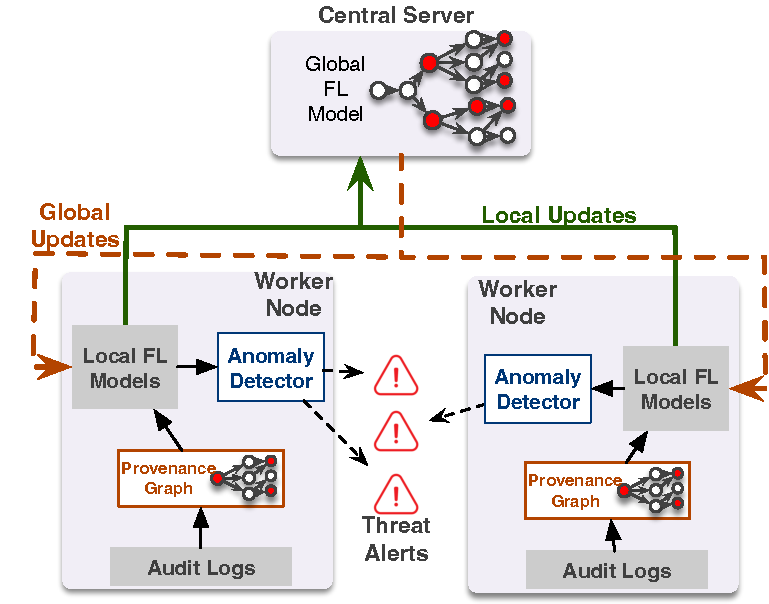
\includegraphics[width=0.40\textwidth]{fig/arch.pdf}
    \caption{Workflow of our proposed decentralized CDR.}
    \label{fig:arch}
    % \end{figure}
  \end{wrapfigure}

  Our proposed CDR system, \Sysa, will incorporate this FL aggregation to create an accurate and scalable anomaly detector, as illustrated in Figure~\ref{fig:arch}. During the training phase, we will use FL to train GNN models across distributed worker nodes using benign log data, allowing the system to learn patterns of normal behavior without centralizing sensitive logs. This decentralized approach enables each worker node to contribute to the model while retaining data locally, building a comprehensive understanding of typical system activities across diverse environments. In the detection or runtime phase, these trained models will then analyze incoming log data for deviations from learned benign patterns, flagging anomalous activities that may indicate potential threats.
  
  To handle scalability and complexity, we will explore GNN architectures such as GraphSAGE~\cite{hamilton2017inductive} for inductive learning on large graphs, and ChebNet~\cite{tang2019chebnet} to generalize convolutions across graphs, which is critical for processing large-scale data. Attention mechanisms from Graph Attention Networks~\cite{velivckovic2017graph} will dynamically weigh node importance, enhancing embedding precision. Spatio-Temporal Graph Networks~\cite{yu2017spatio} will capture evolving patterns over time, addressing the temporal aspect of system logs. For model efficiency within the FL setup, we will implement adaptive learning rate techniques and asynchronous updates~\cite{ye2022eco}. Additionally, to reduce processing delays common in traditional GNN models, we will adopt efficient architectures like GraphSAGE and ChebNet, which enhance processing speed and scalability in large cloud environments. Through these optimizations, \Sysa aims to provide a high-performance, scalable solution for cloud-native anomaly detection.



\eval  We will evaluate system scalability by incrementally increasing the number of worker nodes and data volume, monitoring key metrics such as throughput, latency, and resource utilization (CPU and memory) across diverse network environments. For performance benchmarking, we will use DARPA datasets along with additional, systematically generated benign and malicious datasets. Malicious data will be created using MITRE Caldera~\cite{caldera} and Infection Monkey~\cite{infectionmonkey}, tools designed to emulate a broad range of APTs scenarios by replicating complex attack patterns and testing across diverse network configurations. To generate realistic benign logs, we will employ Generative Adversarial Networks (GANs)~\cite{graphrnn,graphvae} which capture the structure and dynamics of typical enterprise logs, producing synthetic, diverse benign data with essential characteristics for effective CDR evaluation.





\Task{\Sysb: An AI-Enhanced System for Efficient Alert Investigation in SOCs}{task:2} SOC teams often rely on investigation queries in languages like Kusto Query Language (KQL) to analyze alerts from CDR systems, a process that can be time-consuming and demands significant expertise~\cite{esgstudy,alahmadi202299socstudy}. Automating the conversion of investigation prompts into precise SIEM queries could improve SOC efficiency, enabling analysts to focus more on responding to threats. Current automated tools, like Microsoft's Copilot for Security (CFS), have shown limitations in accuracy. For example, when tasked to retrieve all external emails sent by a user on a specific date, CFS returned only five results due to syntax errors, whereas manual analysis identified 17 relevant emails~\cite{microsoftseccopilot}. This highlights the need for a solution that can consistently generate accurate SIEM queries to enhance alert investigations.



\proposedwork{To address the above challenges, we develop an LLM-based assistant, \Sysb, to generate effective investigation queries for SIEM systems from SOC prompts.} Inspired by structured methodologies that improve language model reasoning on complex tasks~\cite{ouyang2023structured}, \Sysb follows a systematic workflow that enhances SOC response efficiency and accuracy. The approach involves generating structured instructions, followed by iterative query construction and refinement phases to produce high-quality, deployable query outputs tailored to SOC requirements.

\begin{itemize}[leftmargin=*,noitemsep,topsep=-1pt]
    
    \item \textit{Structured Instruction Generation}: The process begins with \Sysb generating a structured instruction set based on the SOC investigation prompt. This structured prompt guides the LLM, outlining clear parameters such as required data fields, relevant event types, specific entities (e.g., user IDs, IP addresses), and contextual filters. These instructions serve as a foundational blueprint, helping the LLM interpret the query requirements accurately and establish the investigation’s objectives.
    
    \item \textit{Structured Query Generation and Step-by-Step Reasoning}: Using the structured instruction, the LLM constructs an initial investigation query, breaking down the prompt into logical steps. This phase involves identifying and assembling the necessary building blocks—such as data fields, operators, functions, and relationships -- into a coherent query flow. The LLM applies step-by-step reasoning to ensure that each component aligns with the investigation's intent, translating prompt instructions into specific SIEM operations like `where` and `join` clauses, and verifying that the syntax and logic adhere to SIEM standards.

    \item \textit{Query Validation and Confidence-Based Refinement}: After generating the preliminary query, \Sysb initiates a confidence-based review and refinement process. Each part of the query is evaluated for accuracy and logical consistency, with confidence scores assigned to each component. Any segments with low confidence undergo iterative refinement, where \Sysb revisits the structured instruction and query components, making adjustments to improve performance and coherence. This feedback loop enables \Sysb to iteratively enhance the query until it meets predefined accuracy and efficiency thresholds.
    
    \item \textit{Final Output Generation}: Upon completing the confidence-based refinement, \Sysb produces a finalized investigation query that is ready for SOC deployment. The resulting query is both context-aware and optimized for effective alert investigation, allowing SOC teams to quickly differentiate between false alarms and genuine threats without extensive manual input.
    

\end{itemize}

This structured, multi-phase approach ensures that \Sysb provides SOC teams with precise, contextually accurate queries, streamlining alert investigation workflows and reducing dependency on manual query formulation. By incorporating step-by-step reasoning and iterative refinement, \Sysb enables SOCs to handle alerts more effectively and respond to threats with high confidence and minimal error.

\eval The evaluation of \Sysb’s query generation will focus on accuracy, efficiency, and real-world applicability. Accuracy will be measured by comparing \Sysb-generated queries to those created by SOC analysts, using precision and recall metrics to assess the retrieval of relevant log data without excess noise. Efficiency will be evaluated by calculating time saved in query formulation, comparing \Sysb’s speed to that of human analysts to gauge its impact on SOC response times. To test real-world applicability, \Sysb will be applied to SOC-like prompts using DARPA datasets \cite{darpatc, darpaoptc} or similar logs from controlled environments, analyzing its handling of prompts with varied complexity. We will track false positive and negative rates in incident detection to assess performance across different scenarios.




\begin{figure}[t!]
    % \begin{wrapfigure}{R}{.50\linewidth}
        \centering 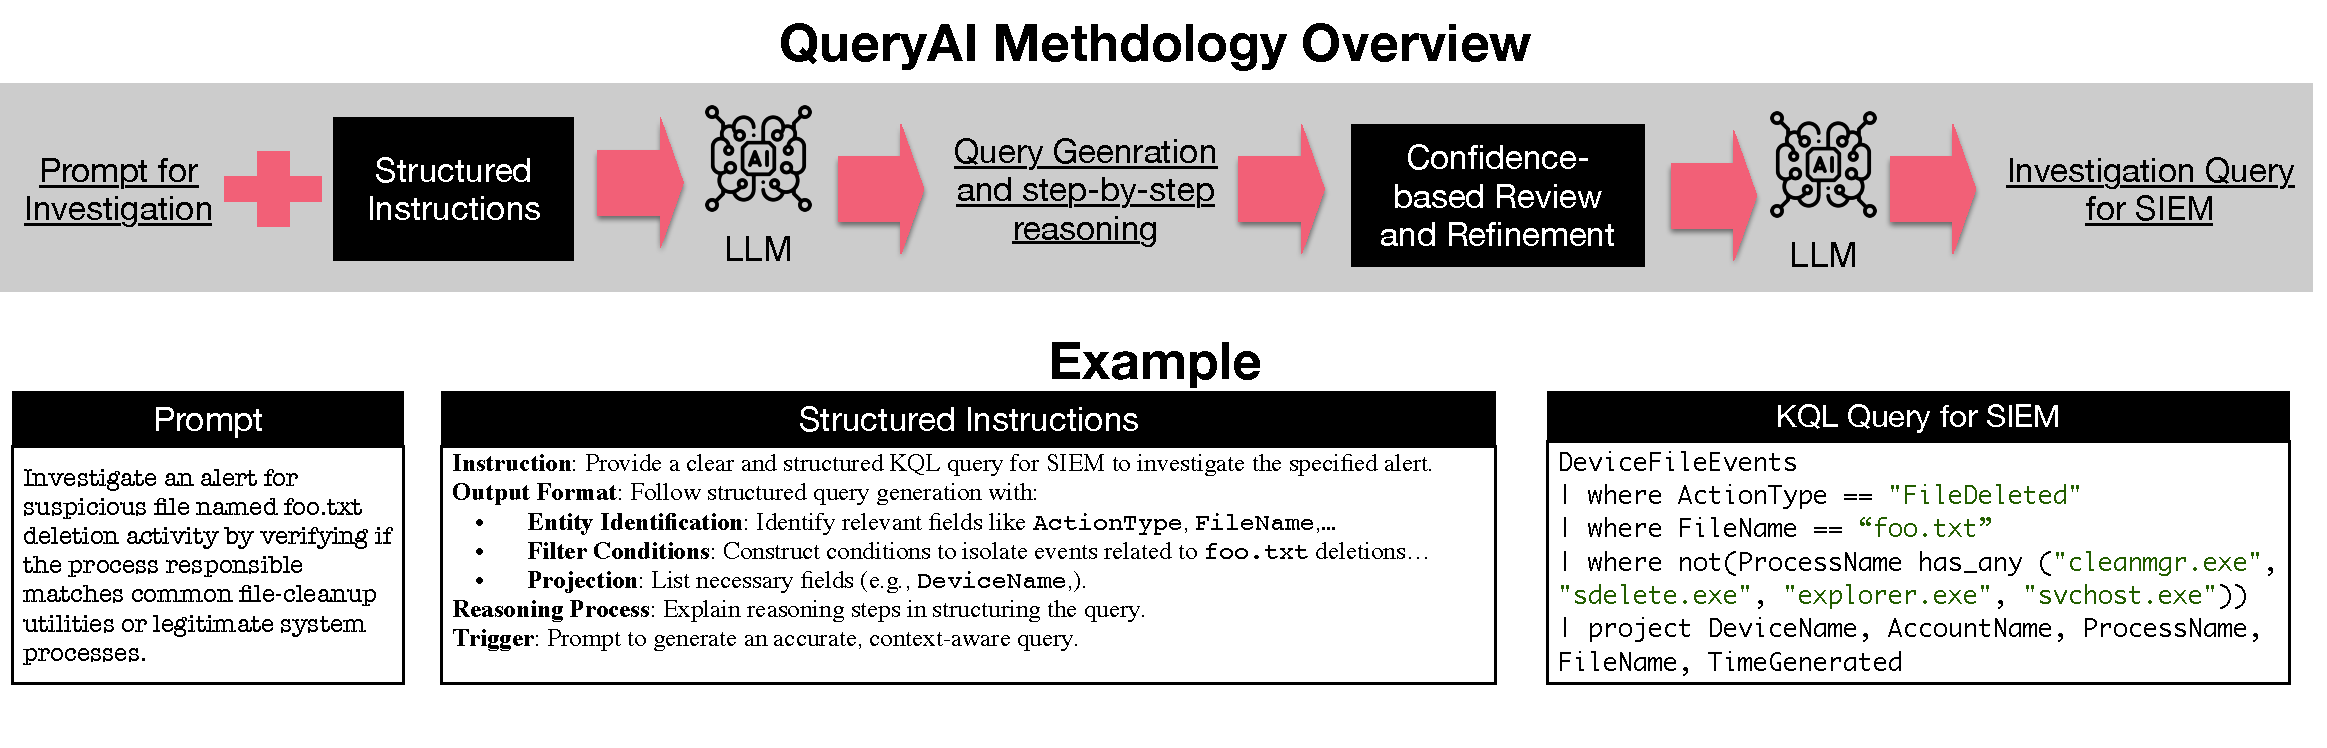
\includegraphics[width=0.99\textwidth]{fig/kql-query.pdf}
        \caption{An in-depth illustration of the QueryAI framework for investigation. The workflow begins with structured instructions that prompt the LLM to generate a KQL query tailored to investigate suspicious file deletion activity. The process initiates with the query generation and step-by-step reasoning stage, forming the initial query structure. Each generated query undergoes a confidence-based review and refinement process, with confidence scores guiding iterative adjustments. This cycle is repeated until reaching a refined query that meets accuracy and relevance criteria.}
        \label{fig:kqlquery}
    % \end{wrapfigure}
\end{figure}


\section*{Expected Results}

A Ph.D. student, under the guidance of PI Hassan at the University of Virginia, will work on this project to bridge academic research with industry needs by advancing CDR systems through scalable, decentralized threat detection and response methods tailored for cloud environments. The project's timeline is outlined in Figure~\ref{fig:sched}. This research will yield several key outcomes:

\begin{wrapfigure}{R}{.45\linewidth}
    % \begin{figure}[t!]
    \centering 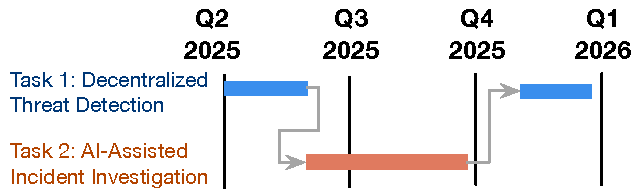
\includegraphics[width=0.45\textwidth]{fig/schedule-e2e.pdf}
    \caption{Anticipated timeline of the proposed work.}
    \label{fig:sched}
    % \end{figure}
    \vspace{-2ex}
  \end{wrapfigure}

\begin{itemize}[leftmargin=*,noitemsep,topsep=-1pt]
    \item We will develop \Sysa, a cloud-native, decentralized detection system using FL and GNNs to process logs locally, reducing centralized data transfers. Deliverables for \Sysa, available by Q3 2025, include the FL-GNN integration codebase, pre-trained model weights,  optimized GNN architectures, and initial datasets of benign and adversarial logs to serve as benchmarks for the cloud security community.

    \item We will design \Sysb, an AI-driven SOC assistant that automates investigation query generation from SOC prompts, enhancing alert investigation. \Sysb will leverage a pre-trained LLM and threat intelligence for context-aware query generation, enabling SOCs to investigate alerts without raw log access. The release, scheduled for Q4 2025, includes \Sysb's codebase,and a technical report.
    
    \item Comprehensive deliverables, including curated datasets, code, model weights, and documentation, will be available by Q1 2026. Findings, methodologies, and benchmarks on scalability and accuracy will be presented at IEEE S\&P, USENIX Security, and ACM CCS. We will also offer hands-on tutorials and maintain an online repository to support ongoing updates and community contributions.
    
\end{itemize}
    
\section*{Funds Needed}

We request cash funding to cover personnel costs, including \$60,000 for one year's salary for a graduate student (covering stipend, tuition, health insurance) and \$15,000 for one month of summer salary for PI Hassan. Additionally, we seek \$25,000 in AWS Promotional Credits to manage computational and storage demands using Amazon EC2 and Amazon S3. Our project involves running experiments on the p3.2xlarge instance for ML tasks at \$3.06 per hour, 24 hours a day, 5 days a week, totaling \$17,625.60 annually for EC2. We also require secure storage of 5 TB on Amazon S3 for storing and sharing system logs produced in Task~\ref{task:1}, with operational costs totaling \$2,580 annually. This \$25,000 in AWS Promotional Credits will also accommodate potential fluctuations and unforeseen costs.





% \PP{Task 2: Privacy-aware HIDS} The main task for this phase is a privacy-preserving intrusion detection system built upon a FL framework integrated with a GNN model. The system will employ an LDP module to add Laplacian noise to gradients during model updates, ensuring privacy protection. At a high level, the technical execution involves preprocessing the provenance graphs, generating adjacency matrices, and creating node feature matrices, followed by adjacency matrix normalization. Each host will initialize its local GNN model with the same initial parameters. During training, the GNN performs forward passes through the neural layers, using the ReLU activation function and the weight matrix for each layer. The model parameters' gradients will be computed via backpropagation, and model updates will be performed using an optimization algorithm, such as SGD. The updated models will then be sent to a central server for aggregation, before being distributed back to the hosts.



% \PP{Task 3: Incident Response}  This task aims to harness insights from the GNN-based intrusion detection model to formulate efficient alert triage and response methods. Initially, an {\it alert prioritization algorithm} will be designed, factoring in threat nature, system vulnerability, and potential attack consequences, ensuring resources are directed at the most crucial threats. Following that, we will devise {\it automated incident response techniques} to automate threat mitigation steps. Emphasizing human-centric decision-making, a {\it decision support system} will be created, offering analysts actionable recommendations based on the GNN-based model outputs. Visualization tools will make complex graph data analysis intuitive.




